\chapter{Comparing software variability across and within fMRI analysis packages}
\label{ch:c3}

Ali Salari\footnote{\label{note1}Department of Computer-Science and Software Engineering, Concordia University, Montreal, Canada},
Yohan Chatelain\textsuperscript{\ref{note1}},
Alexander Bowring\footnote{\label{note3}Li Ka Shing Centre for Health Information and Discovery, Nuffield Department of Population Health,\\ Big Data Institute, University of Oxford, Oxford, UK},
Camille Maumet\footnote{\label{note4}Inria, Univ Rennes, CNRS, Inserm, IRISA UMR 6074, Empenn ERL U 1228, Rennes, France},
Gregory Kiar\footnote{\label{note2}Center for the Developing Brain, Child Mind Institute, New York, NY, USA},
Tristan Glatard\textsuperscript{\ref{note1}}
\\ \\ \\
To be submitted to:

Human Brain Mapping (HBM) journal

\newpage
\noindent\fbox{%
\parbox{\textwidth}{%
\setstretch{1.5}
\textbf{Abstract}

Variability has been broadly observed in functional MRI analyses as a
result of software differences both between and within analytic tools.
However, the relationship between within-tool and between-tool software
variabilities for a given analysis is unclear. Within-tool variability has multiple origins
including variations in algorithms, parametrizations, and
low-level software dependencies. We focus on the effects resulting from software dependencies --- 
in particular due to operating system and other infrastructural updates --- as they often remain unnoticed 
while algorithms and parametrizations are more controllable.
We extended
a previous comparison of fMRI analysis software libraries (namely FSL,
AFNI, and SPM) and related the observed differences to within-tool
software variability simulated using Monte-Carlo arithmetic. In group
analyses, we found that
between-tool software variability was consistently larger than within-tool software
variability. In subject analyses, within-tool software variability
approached between-tool software variability in some regions for some subjects.
Interestingly, the brain masking instability was triggered by both within- and between-tool
software variabilities.
Our findings motivate the continued investigation of within-tool
software variability in neuroimaging, and position it as a possible proxy
for studying some of the arbitrary between-tool software variations for
subject-level analyses.
\\
}%
}
\newpage

\renewcommand\fbox{\fcolorbox{black}{white}}
\section{Introduction}

Recent explorations of the analytical flexibility in brain imaging across
tools, platforms, or teams, have demonstrated unexpected variability in
results, even when analyzing identical data~\cite{botvinik2020variability}. Possible explanations for
such discrepancies include methodological flexibility~\cite{carp2012plurality} and software
variability, the focus of this paper. A recommendation to address this
variability is to adopt a ``multiverse" approach that analyzes the same
dataset multiple times in different software environments, and ultimately
conclude from the resulting set of outcomes. However, the range of
analytical conditions to be included in such multiverse analyses remains
poorly defined, both because of the boundless set of tools and
configurations, and that the precise causes of software variability remain
unclear. This lack of clarity is in part because fMRI analyses depend on
complex software stacks that leverage low-level libraries provided by the
operating system (e.g., mathematical functions), general scientific
computing methods (e.g., optimization toolboxes), and specific fMRI
analysis tools (e.g., spatial image normalization methods). At each level,
conceptual and implementation differences across experiments may each
create substantial variability in the analysis outcomes.

As a result of these factors, the variability resulting from the use of
different fMRI analysis tools implementing similar analytical approaches
(between-tool software variability), or different versions of the same tool,
 can reach worrying magnitudes. For instance, the
study in~\cite{bowring2019exploring} compared the results produced by the
three main fMRI analysis toolboxes, namely SPM~\cite{penny2011statistical},
AFNI~\cite{cox1996afni} and FSL~\cite{jenkinson2012fsl}, using similar
pipelines. It reported limited similarity between the activation clusters
produced by these tools, measured by Dice coefficients ranging from 0.0 to
0.769, where 0 indicates non-overlapping
clusters and 1 means identical clusters. More recently, the work
in~\cite{Li2021.12.01.470790} also showed a low similarity between the
results produced by five different tools (ABCD~\cite{feczko2021adolescent},
CCS~\cite{xu2015connectome}, CPAC~\cite{craddock2013towards}, DPARSF~\cite{yan2010dparsf},
fMRIPrep~\cite{esteban2019fmriprep}) and identified the main
factors contributing to these differences. The magnitude of the highlighted
differences suggest that between-tool software variability may be playing a critical
role in the reproducibility of an fMRI analysis overall. 

The variability resulting from differences in lower-level software
libraries (within-tool software variability) has also been quantified in fMRI. The
study in~\cite{Glatard2015} mentions a low similarity between the activation clusters
produced by FSL using different versions of the GNU/Linux system, measured
by Dice coefficients ranging from 0.0 to 1.0, covering the full spectrum of
possible similarities. This variability resulted from updates in the GNU
mathematical library and can be properly simulated by introducing small
numerical perturbations on the results returned by mathematical functions~\cite{salari2021accurate}.
Here again, these observations could partly explain the differences
reported in~\cite{botvinik2020variability}.

The relationship between within- and between-tool software variability are poorly
understood, but could play an important role in the construction of
multiverse study environments. Importantly, if associations exist between
these two types of variability, they may both originate to some degree from
the inherent instability of brain activity estimation from BOLD signal
variations, and shed light on the numerical confidence of results. Under
this hypothesis, small perturbations introduced by low-level software
updates could trigger effects correlated with those created by tool
variations.

This paper investigates the relationship between numerical stability --- used
as a proxy for within-tool software variability --- and between-tool software variability
through two main questions:
\begin{enumerate}
\item what is the relative magnitude of within- and between-tool software variability, and
\item is there an association between within- and between-tool software variability.
\end{enumerate}

We address these two questions by reproducing the study in~\cite{bowring2019exploring} and
extending it with the addition of numerical perturbations of controlled
magnitude.

\section{Materials and Methods}

\subsection{fMRI analysis \& Dataset}

We replicated the analysis described as study `ds000001'
in~\cite{schonberg2012decreasing}, relying on the data publicly available
in OpenNeuro at \url{https://openneuro.org/datasets/ds000001} and using
three widely-used software packages for fMRI data processing, namely FMRIB
Software Library (FSL)~\cite{jenkinson2012fsl}, Analysis of Functional
NeuroImages (AFNI)~\cite{cox1996afni}, and Statistical Parametric
Mapping (SPM)~\cite{penny2011statistical}. We selected this dataset because
comparable analysis pipelines implemented in FSL, AFNI and SPM were already
publicly available and extensively described in~\cite{bowring2019exploring}.
Furthermore, the work in~\cite{bowring2019exploring} already evaluated the
effect of tool variability for this dataset, which we intended to
extend with the present quantification of within-tool variability.

In the selected study, 16 healthy adult subjects participated in the
balloon analog risk task~\cite{lejuez2002evaluation} to measure risk-taking
behavior over three scanning sessions~\cite{schonberg2012decreasing}. We
reused the preprocessing, first-level, and second-level analyses
implemented by~\cite{bowring2019exploring} consistently across all three
software packages. Table~\ref{table:pipeline-steps}, adapted from~\cite{bowring2019exploring},
summarizes the analytical steps in each
pipeline.

%%%%%%%%%% Summary of statstics %%%%%%%%
\setlength{\tabcolsep}{4pt}
\begin{table}[h]
  \centering
  \begin{tabular}{|c|l|c|c|c|}
    \hline
    %        \multirow{2}{*}{} & \multicolumn{1}{c}{Thresholded}& & \multicolumn{1}{c}{Unthresholded}& \\
    \multicolumn{2}{|c|}{} & FSL                                & AFNI       & SPM                     \\
    \hline
    {Preprocessing}        & {Motion Correction}                & \checkmark & \checkmark & \checkmark \\
    {}                     & {Segmentation}                     &            &            & \checkmark \\
    {}                     & {Brain Extraction (Anatomical)}    & \checkmark & \checkmark & \checkmark \\
    {}                     & {Brain Extraction (Functional)}    &            & \checkmark &            \\
    {}                     & {Intra-subject Coregistration}     & \checkmark & \checkmark & \checkmark \\
    {}                     & {Inter-subject Registration}       & \checkmark & \checkmark & \checkmark \\
    % {}                     & {Analysis Voxel Size}              & \checkmark & \checkmark & \checkmark \\
    {}                     & {Smoothing}                        & \checkmark & \checkmark & \checkmark \\
    \hline
    {First-level}          & {Model Specification}              & \checkmark & \checkmark & \checkmark \\
    {}                     & {Inclusion of 6 Motion Parameters} & \checkmark & \checkmark & \checkmark \\
    {}                     & {Model Estimation}                 & \checkmark & \checkmark & \checkmark \\
    {}                     & {Contrasts}                        & \checkmark & \checkmark & \checkmark \\
    \hline
    {Second-level}         & {Model Specification}              & \checkmark & \checkmark & \checkmark \\
    {}                     & {Model Estimation}                 & \checkmark & \checkmark & \checkmark \\
    {}                     & {Contrasts}                        & \checkmark & \checkmark & \checkmark \\
    {}                     & {Second-level Inference}           & \checkmark & \checkmark & \checkmark \\
    \hline
  \end{tabular}
  \caption{Software processing steps (adapted from~\cite{bowring2019exploring}).}
  \label{table:pipeline-steps}
\end{table}


\subsection{Within-tool software variability simulation with Fuzzy Libmath}

We simulated within-tool software variability by introducing 
numerical noise in the analyses using
Fuzzy Libmath~\cite{salari2021accurate}, a version of the GNU
mathematical library (libmath) instrumented with Monte-Carlo arithmetic.
Monte-Carlo arithmetic simulates numerical errors
by introducing a controlled amount of noise in floating-point
operations through the following perturbation~\cite{Parker1997-qq}:

\begin{equation} \label{eq:mca_inexact}
  inexact(x) = x + 2^{e_x-t}\xi,
\end{equation}
where $e_x$ is the exponent in the floating-point representation of $x$,
$t$ is the virtual precision (the number of unperturbed bits in the
mantissa of $x$), and $\xi$ is a random uniform variable of
$(-\frac{1}{2}, \frac{1}{2})$. We introduced the perturbation using
Verificarlo~\cite{denis2015verificarlo}, an LLVM compiler supporting Monte-Carlo
arithmetic and other types of numerical instrumentations.

We loaded the instrumented libmath functions in the pipeline using
LD\_PRELOAD, a Linux mechanism to force-load a shared library into an
executable. This mechanism allows functions defined in Fuzzy Libmath to transparently
overload the original ones without the need to modify or recompile the
analysis pipeline.

Fuzzy Libmath introduces numerical perturbations in the values returned by
mathematical functions but not in their input values or within their
implementation. This is done by wrapping the original functions and
applying function \texttt{inexact} to their returned values.
Listing~\ref{algo:wrapper} shows an example of this wrapping for the
\texttt{log} function in single and double precision. In this wrapper, the
original function is called through \texttt{dlsym}, a function that returns
the memory address of a symbol --- in our case \texttt{RTLD\_NEXT}, the
address of the next occurrence of the function in memory. Compiling function wrappers
with Verificarlo instruments the result of the
addition between the original function output and the floating-point zero.

\lstdefinestyle{customasm}{
  belowcaptionskip=1\baselineskip,
  frame=L,
  xleftmargin=\parindent,
  language=[x86masm]Assembler,
  basicstyle=\footnotesize\ttfamily,
  commentstyle=\itshape\color{purple!40!black},
}
\lstinputlisting[caption=Sample wrapper function (C code),
  label=algo:wrapper, style=customasm]{chapters/chapter3/wrapper.c}

In~\cite{salari2021accurate}, Fuzzy Libmath was shown to accurately
simulate the effect of Linux operating system updates in structural
pre-processing pipelines of the Human Connectome Project which are largely based on FSL.
To validate our pipeline instrumentations for the present study, we first verified that non-instrumented
executions of the same pipeline on the same dataset led to identical
results. We also listed the pipeline
library dependencies using the \texttt{ldd} Linux utility and verified that
(1) the tested pipelines were dynamically linked to the GNU libmath library, and
(2) there was no alternative implementation of elementary mathematical functions in the pipeline dependencies.
Finally, we verified that the use of Fuzzy Libmath affected computational results.
  
\subsection{Data processing}

We measured between-tool software variability (BT) by running the pipelines
described in~\cite{bowring2019exploring} with FSL version 5.0.10, AFNI
version 18.1.09, and SPM12 version r7771 executed with GNU/Octave version
5.2. These software versions were identical to the ones used 
in~\cite{bowring2019exploring} except for SPM for which we had to use
a more recent version in order to be able to use it with GNU/Octave
instead of MATLAB to enable mathematical function instrumentation using
Fuzzy Libmath. Indeed, MATLAB uses its own built-in mathematical functions,
which prevents the use of Fuzzy Libmath. In AFNI, we set the number of
threads to 7 even though AFNI executions
in~\cite{bowring2019exploring} were single-threaded. This was meant to
reduce the time overhead resulting from Fuzzy Libmath instrumentation.
All the analyses were conducted on the CentOS 7.3 operating system. The
computations were performed on \href{https://www.computecanada.ca}{Compute
  Canada's} Béluga cluster nodes, each with 2$\times$ Intel Gold 6148 Skylake~@~2.4~GHz
(40 cores/node) CPU and 8~GB of RAM per core. To facilitate portability and reproducibility,
we encapsulated the
above-mentioned software packages in Docker container images based on CentOS 7.3
which we converted to Singularity images to enable running on cluster nodes.

In the IEEE-754 format, a floating-point number $N$ is represented by a sign
bit (s), an exponent (e), and a pseudo-mantissa (m) as:

\begin{equation}
  N = (-1)^s \times 2^E \times (1.m),
\end{equation}
where $E=e-127$ for single precision and $E=e-1023$ for double precision.
In single precision, the pseudo-mantissa has 23 bits and the exponent has 8 bits, whereas in
double precision the pseudo-mantissa has 52 bits and the exponent has 11 bits.
Machine error, the smallest absolute difference between two
floating-point numbers that can be represented, is in general $2^{-24}\times e$ in
single precision and $2^{-53}\times e$ in double precision.
We simulated machine error by introducing the random perturbation defined
in Equation~\ref{eq:mca_inexact} at the virtual precision of $t=24$~bits for single-precision
values and $t=53$~bits for double-precision ones. The perturbed pseudo-mantissa
is obtained by extending the size of the original pseudo-mantissa, applying the perturbation
at the desired virtual precision, and rounding the perturbed result back to the original precision.
We simulated within-tool software variability (WT) by running the same analyses 10
times using Fuzzy Libmath with a virtual precision of $t=53$~bits for
double-precision values and $t=24$~bits for single-precision values. 
Perturbations were applied at the same magnitude of floating-point precisions during the pipeline execution
regardless of what it corresponds to.
These values were chosen such that the numerical perturbation affects all the pipeline steps and simulates
machine error originating from software, hardware, and operating system changes.
The resulting samples are equally plausible estimates of
the true numerical result at the precision used by the pipelines. 

We evaluated BT for thresholded as well as unthresholded
group-level and subject-level t-statistic maps by computing the
differences of t-statistic maps across tools. For WT, we computed the
average difference across the 10 Fuzzy Libmath samples.

Further, from the thresholded maps, we determined regional instability
between activation clusters in the 360 regions in the Human Connectome
Project Multi-Modal Parcellation atlas version 1.0
(HCP-MMP1.0)~\cite{glasser2016multi}. For BT, we considered a region
unstable for a pair of tools if it contained activated voxels for a tool
but not for the other one. For WT, we considered a region unstable for a
pair of tools (A, B) if for tool A or tool B it contained activated voxels only for some Fuzzy Libmath
samples.

\section{Results}
The scripts, Docker images, and derived datasets that were used to reproduce the results are available
in our GitHub repository at \url{https://github.com/big-data-lab-team/fuzzy-neurotools}.

\subsection{Validation of replication}

We verified the correctness of our analyses by comparing our unperturbed
t-statistic group maps with the ones obtained
in~\cite{bowring2019exploring}. For FSL, we found
strictly identical results with the same MD5 checksums. For SPM, the files (as measured by MD5 checksums) were different but differences
were visually unnoticeable. For AFNI, the overall patterns of activations were preseved
, however, differences were noticeable visually.
The observed differences remained small (see Supplemental Material~\ref{sec:supp-repro}), and might be due to the use of
GNU/Octave vs MATLAB in SPM, and of multithreading in AFNI. We performed visual quality control of the AFNI
and SPM results for each individual subject and confirmed that T1-weighted images were
correctly skull-stripped and registered to the MNI template.

\subsection{In the group analysis, BT was larger than WT}

Table~\ref{table:pipeline-stats} presents summary statistics for variability in the
group-level t-statistic.
Mean of differences in t-statistic maps was centered around zero for BT and WT
in both thresholded and unthresholded maps (t-test p~\textless~$10^{-5}$).
However, for each tool pair (A, B), BT variability was
significantly larger than WT in tool A or B,
with an order of magnitude larger standard deviation of differences 
in both thresholded and unthresholded maps, 
(Wilcoxon signed-rank test and t-test p~\textless~$10^{-5}$).
These global differences were confirmed by Bland-Altman plots showing a
clear dominance of BT over WT
(Figure~\ref{fig:unthresh-maps}-\textbf{A},\textbf{B}).
In addition, results show that BT and WT were not correlated across voxels
(Pearson's r $\approx 0$, p$< 10^{-5}$, Figure~\ref{fig:unthresh-maps-corr}).
% Interestingly, the correlation appears driven by a set of voxels exhibiting comparable BT and
% WT values located around the identity line in Figure~\ref{fig:unthresh-maps}D, which, however, did not seem to have
% any spatial consistency.

\setlength{\tabcolsep}{5pt}
\begin{table}[h]
  \centering
  \begin{tabular}{cccccc|cc}
    \toprule
                      &              & \multicolumn{4}{c|}{Group map}  & \multicolumn{2}{c}{Subject maps}                                                                     \\
    \multirow{2}{*}{} & {}           & \multicolumn{2}{c}{Thresholded} & \multicolumn{2}{c|}{Unthresholded} & \multicolumn{2}{c}{Unthresholded}                               \\
    % \cmidrule{3-8}
    {}                & {}           & $\mu$                           & $\sigma$                           & $\mu$                             & $\sigma$ & $\mu$ & $\sigma$ \\
    \midrule
    \rowcolor{lightgray!50}
    {Between Tools}   & FSL vs. SPM  & -0.845                           & 2.639                              & -0.052                             & 1.122    & -0.059 & 0.911    \\
    \rowcolor{lightgray!50}
    {(BT)}            & FSL vs. AFNI & -0.871                           & 3.216                              & 0.048                             & 1.405    & 0.027 & 1.097    \\
    \rowcolor{lightgray!50}
    {}                & AFNI vs. SPM & 0.426                           & 3.214                              & -0.113                             & 1.543    & -0.104 & 1.208    \\
    {Within Tool}     & FSL          & -0.397                           & 1.218                              & -0.020                             & 0.189    & 0.017 & 0.207    \\
    {(WT)}            & SPM          & 0.142                           & 1.035                              & 0.000                             & 0.139    & 0.000 & 0.126    \\
    {}                & AFNI         & -0.045                           & 1.282                              & 0.000                             & 0.373    & 0.000 & 0.355    \\
    \bottomrule
  \end{tabular}
  \caption{Voxel-wise mean and standard deviation of BT and WT variability in t-statistic maps.}
  \label{table:pipeline-stats}
\end{table}


\begin{figure*}[ht]
  \centering
    % \includegraphics[width=.9\textwidth]{figures/plots/Bland-Altman/with-masking/unthresh-gl-frame.png}
    \includegraphics[width=.9\textwidth]{chapters/chapter3/figures/unthresh-gl-frame.png}
    \caption{\textbf{A} and \textbf{B}: Bland-Altman plots comparing group-level differences computed between tools
    (\textbf{A}) and within tools at machine error (\textbf{B}).}% \textbf{C}: voxel-wise comparison of absolute differences.}
  \label{fig:unthresh-maps}
\end{figure*}

\begin{figure*}[ht]
  \centering
  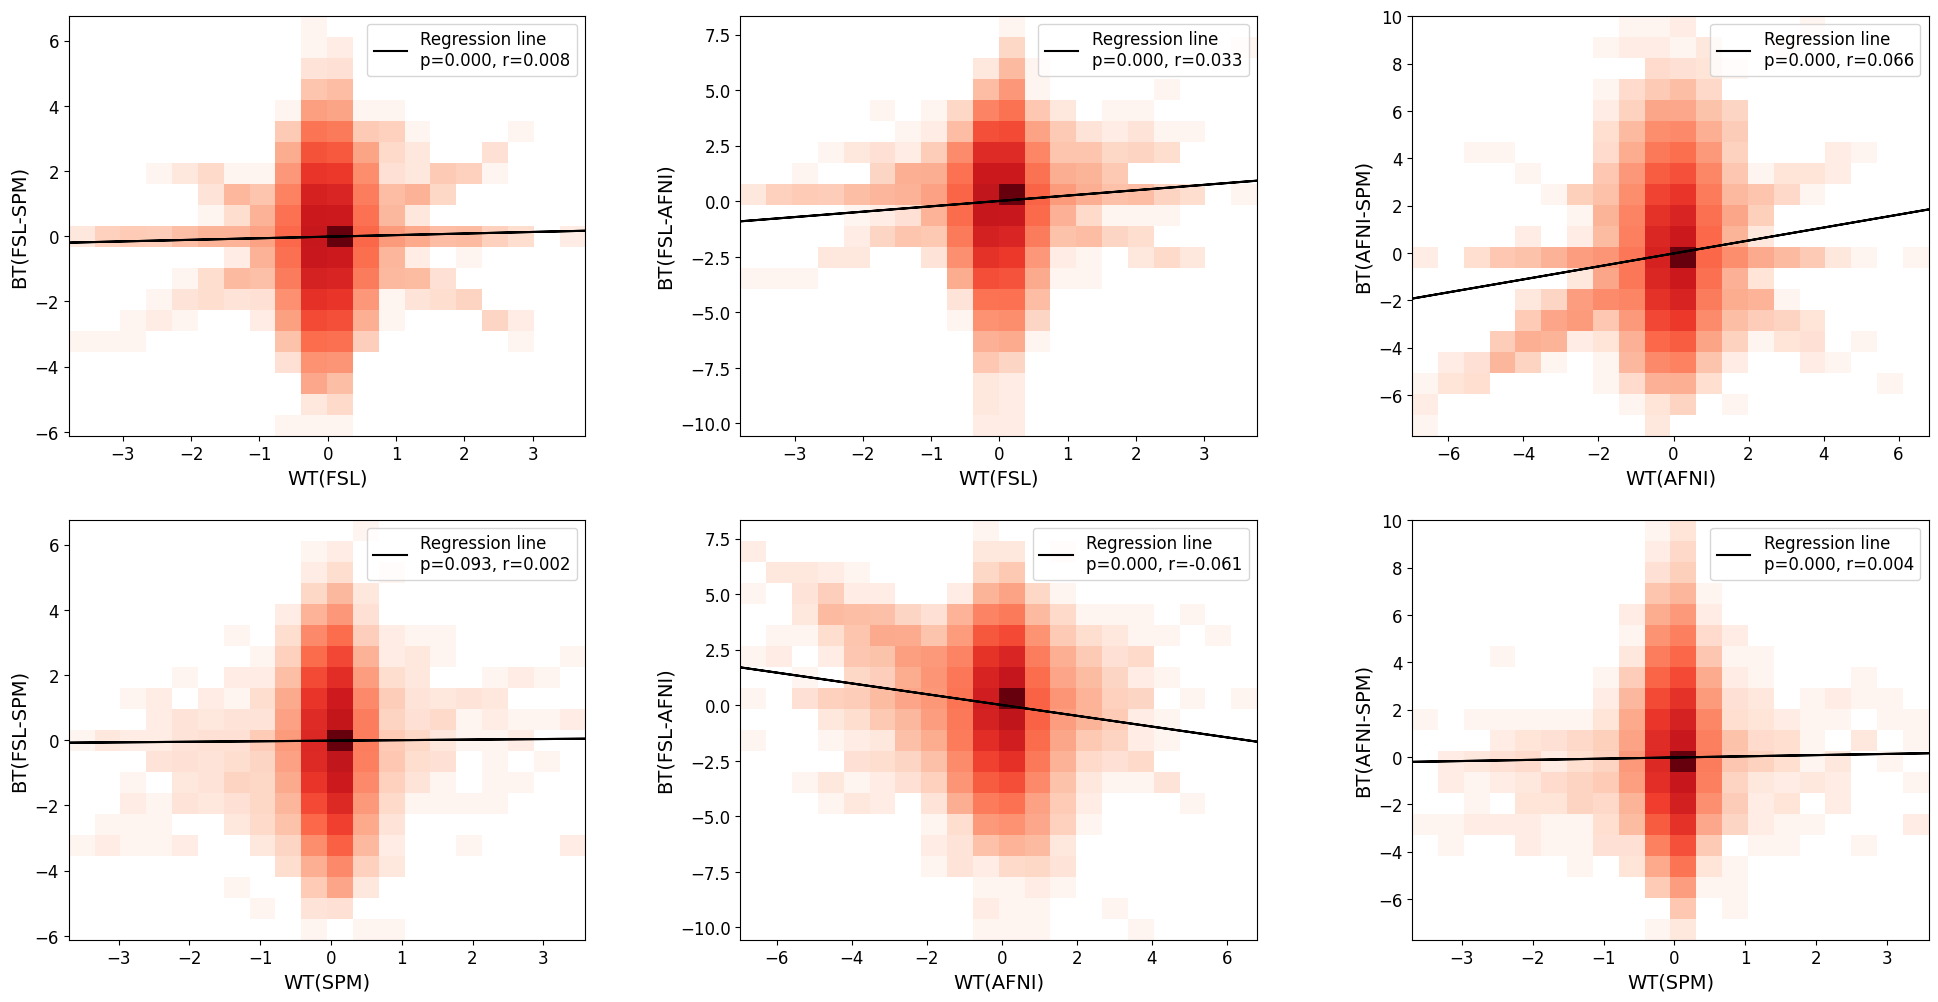
\includegraphics[width=.9\textwidth]{chapters/chapter3/figures/rel-corr-unthresh-with-masking.png}
  \caption{Voxel-wise comparison of group-level differences in BT and WT.}
  \label{fig:unthresh-maps-corr}
\end{figure*}


\subsection{In subject analyses, WT approached BT for some subjects}

Table~\ref{table:pipeline-stats} also presents summary statistics for
subject-level unthresholded t-statistic maps (mean over subjects).
As for group-level maps, the mean of differences in t-statistic maps was
approximately zero centered in both BT and WT (t-test p~\textless~$10^{-4}$ for 13 subjects),
and BT was consistently larger than WT (Wilcoxon
signed-rank test and t-test p~\textless~$10^{-4}$ for 14 subjects).
However, for some subjects and for AFNI, WT approached 
BT in some regions (Figure~\ref{fig:unthresh-maps-sbj},
and see Supplemental Material~\ref{sec:supp-worst-subject}).
% As for the group maps, BT and WT
% showed no correlation across voxels for all subjects
% (r$\approx 0$, p$< 10^{-5}$ for all subjects, see Supplemental Material~\ref{sec:supp-subjects} and~\ref{sec:supp-worst-subject}).

%%%%%%%%%% Var. of Unthresh sbj05%%%%%%%%
\begin{figure*}[ht]
  \centering
  % \includegraphics[width=0.9\textwidth]{figures/plots/Bland-Altman/with-masking/unthresh-sbj05.png}
  \includegraphics[width=0.9\textwidth]{chapters/chapter3/figures/unthresh-sbj05.png}
  \caption{For subject with highest WT variability,
    unthresholded subject-level variability computed between tools (\textbf{A}), and within tools at machine error (\textbf{B}).}
    % and difference between them (\textbf{C}). \camille{If the changes are visible, I think that it would be useful to add the correspondant unthresholded maps for the reader to see where the differences are and what they "look like"}}
  \label{fig:unthresh-maps-sbj}
\end{figure*}

% \subsection{At precision t=17~bits and in FSL, WT approached BT in the group analysis}
% \tristan{We cannot say that from the data that we have.}
% \tristan{Discuss subject-level BA plots.}
% While the previous results were obtained by simulating WT with numerical perturbations 
% at the magnitude of machine error, we also
% evaluated numerical variability across different virtual precisions for FSL
% and found that the virtual precision of t=17 bits minimized the RMSE
% between BT and WT in unthresholded group maps.
% FSL produced unthresholded group maps with $\mu=0.483$ and $\sigma=0.410$ at this virtual precision,
% which was still lower than BT variability
% (Wilcoxon signed-rank test and t-test p~\textless~$10^{-5}$ for all tests).
% However, Figure~\ref{fig:gnp-mni} shows that
% BT and WT reached comparable magnitudes in some regions. BT and WT remained
% moderately correlated at this precision (Pearson's r
% in [0.53, 0.61], p$< 10^{-5}$, Figure~\ref{fig:gnp-mni}-\textbf{B}).

% %%%%%%%%%% plot at precision t=17%%%%%%%%
% \begin{figure*}[ht]
%   \begin{subfigure}[ht]{\textwidth}
%     \centering
%     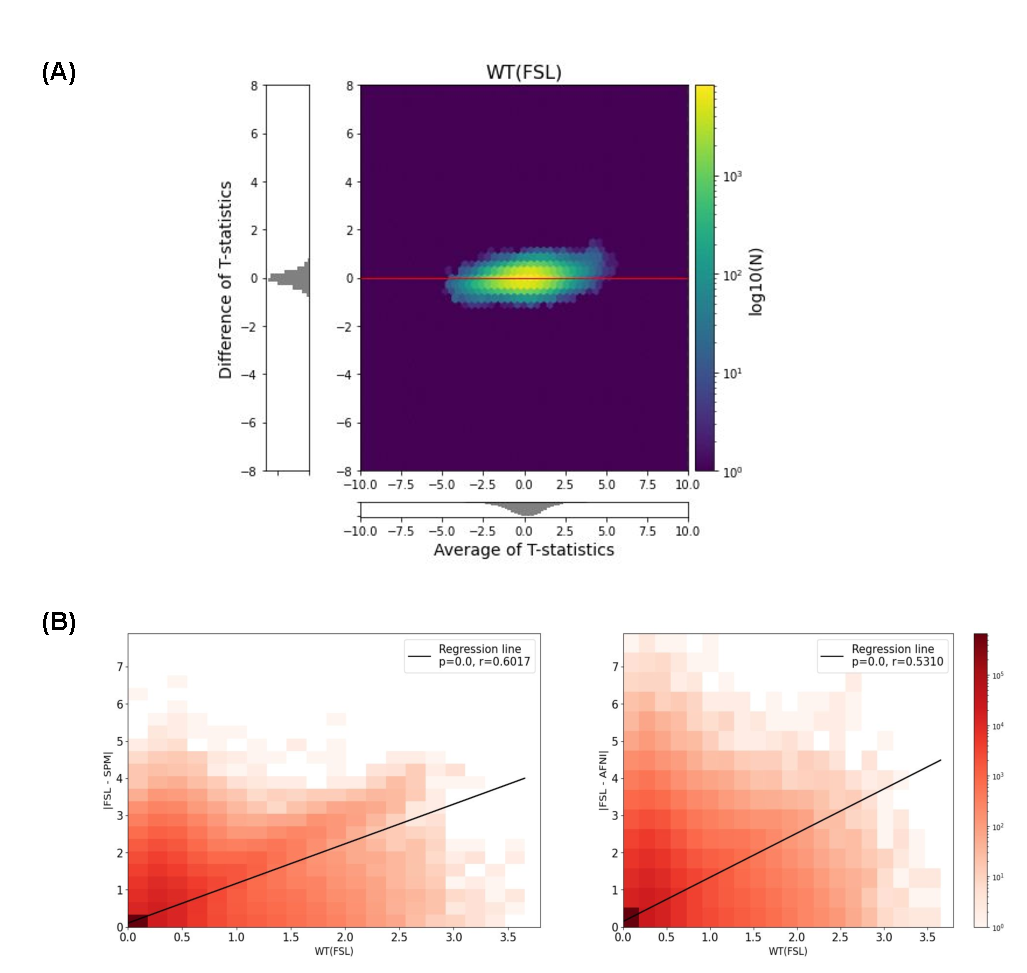
\includegraphics[width=.55\textwidth]{figures/p17-diffs.pdf}
%     % 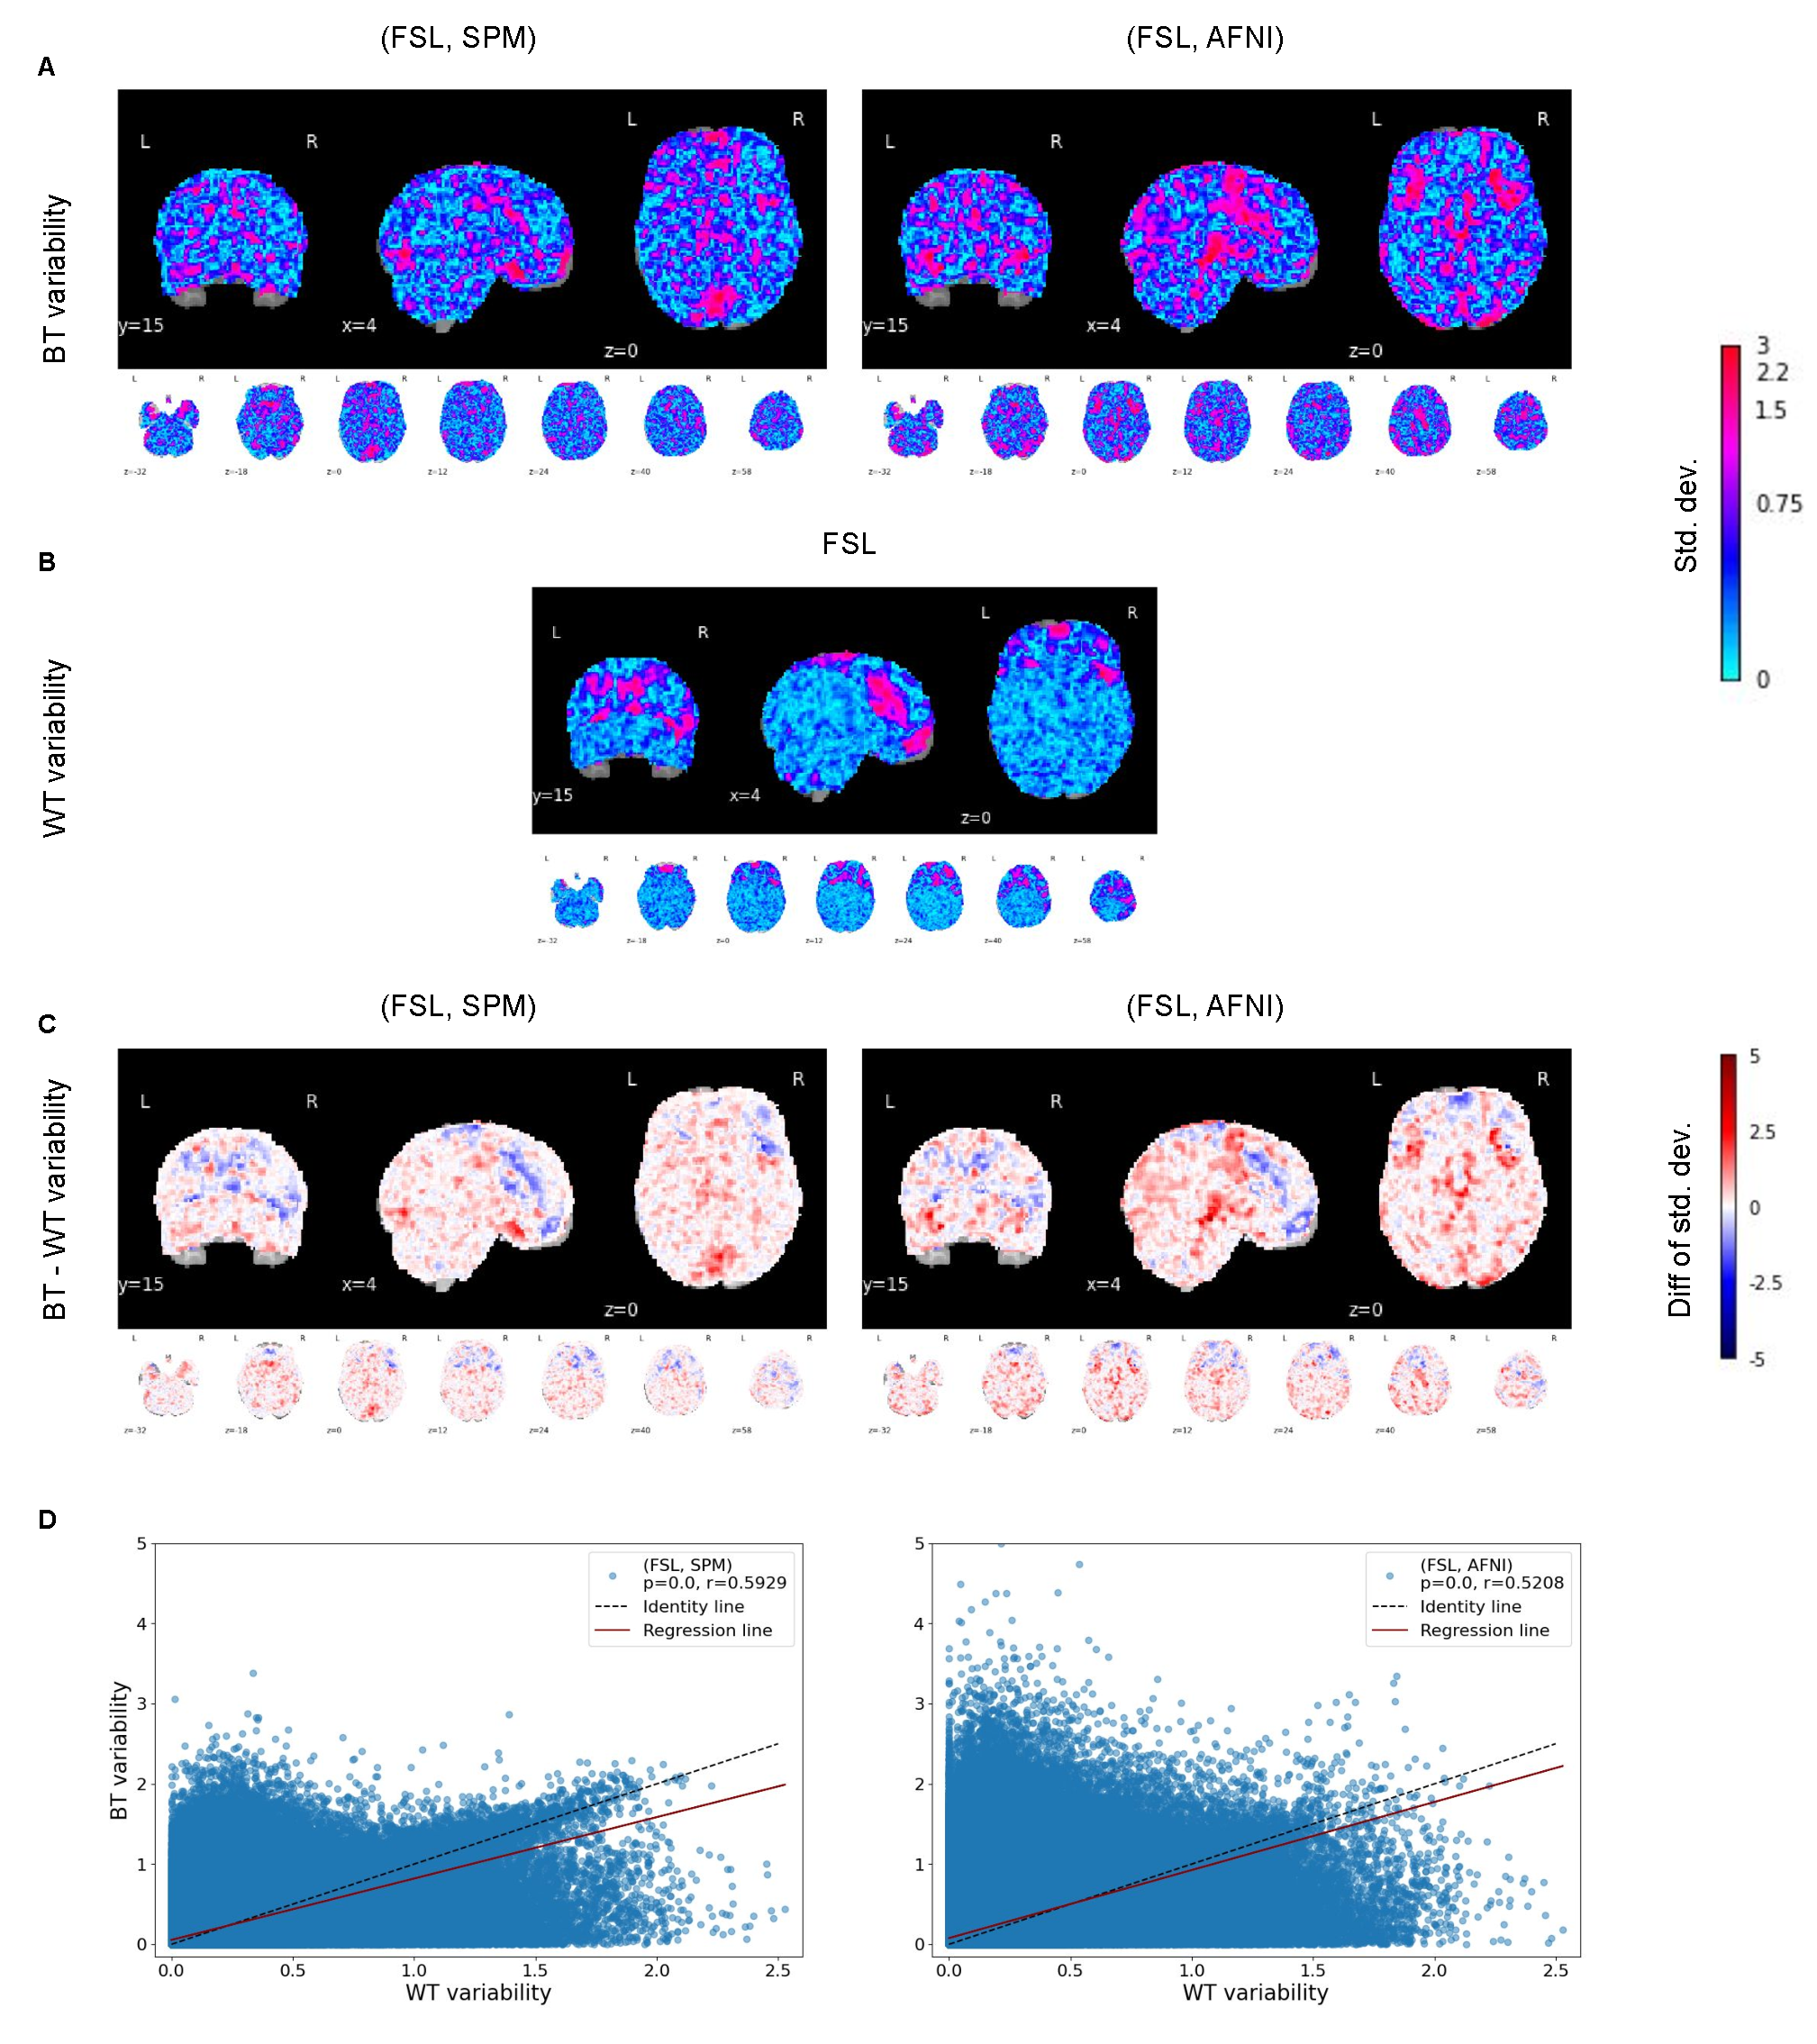
\includegraphics[width=.75\textwidth]{figures/bg_global_precision.pdf}
%     %\caption{Standard deviation of thresholded t-statistics map on template surface}
%   \end{subfigure}
%   %\caption{Standard deviation of thresholded t-statistics map on template surface}
%   \caption{Unthresholded group t-statistics differences computed
%   within tools at the virtual precision of t=17~bits (\textbf{A}),
%   and voxel-wise comparison of absolute differences between BT and WT (\textbf{B}).}
%   \label{fig:gnp-mni}
% \end{figure*}


\subsection{Previous results were confirmed in thresholded group maps}

We also compared BT and WT in thresholded maps since these maps are commonly used instead of unthresholded ones 
to conclude on the activation of specific regions. Thresholding is an unstable operation
that introduced variability at the edges of
active regions for both BT and WT. Except at the edges, BT remained consistently larger
than WT (Figure~\ref{fig:thresh-maps}-\textbf{A},\textbf{B},\textbf{C} and Table~\ref{table:pipeline-stats}). 

Moreover, to compare the effects of BT and WT on the detection of activated
regions, we measured WT instability and BT instability in each region of
the HCP-MMP1.0 parcellation. The confusion matrices in
Figure~\ref{fig:thresh-maps}-\textbf{D} report these instabilities for the
360 tested regions. The average ratio of unstable regions was 26.2\% for BT
and 20.6\% for WT, which confirmed that BT was larger than
WT even in thresholded maps.

Finally, we measured agreement between BT and WT from the confusion
matrices since interpreting the correlation of thresholded maps is
difficult due to the discontinuity introduced by thresholding. 
The average Cohen's kappa score\footnote{$\kappa \leq 0$ denotes chance agreement, $-1 \leq \kappa \leq 1$}
computed from the confusion matrices between WT instability and BT instability was $\kappa=0.2$, indicating
a moderate agreement between WT instability and BT instability consistent with the correlations observed in 
unthresholded maps.

% \gk{again, it feels kind of abrupt and I'm not really sure what this
% section is getting at or how it differs from the previous based on these
% descriptions. Perhaps introduce that thresholding is common, but since it
% makes things discontinuous we study it through aparcellation, etc...}.
% \tristan{better now?}

%%%%%%%%%% Var. of Thresh %%%%%%%%
\begin{figure*}[ht]
  \begin{subfigure}[ht]{\textwidth}
    \centering
    % \includegraphics[width=\textwidth]{figures/act_deact-marked.pdf}
    \includegraphics[width=\textwidth]{chapters/chapter3/figures/act_deact-marked.pdf}
  \end{subfigure}
  \centering
  \caption{\textbf{A},\textbf{B},\textbf{C}: Thresholded group-level
    t-statistic within tools at machine error for FSL (\textbf{A}), SPM
    (\textbf{B}) and AFNI (\textbf{C}). Arrows point to activation clusters
    impacted by both within- and between-tool variability.
     \textbf{D}: Confusion matrices of
    activation instability in BT and WT among the 360 regions of the
    HCP-MMP1.0 parcellation.(with masking)}
  \label{fig:thresh-maps}
\end{figure*}

\subsection{Brain masking instability was triggered by WT and BT}

While the previous results were obtained over the union of t-statistic maps between the pair of tools,
we also computed results in the intersection of maps and found that the brain masking instability was
triggered by both BT and WT.
BT and WT variabilities were consistently smaller than ones with the fixed masks
in both thresholded and unthresholded maps (see Table~\ref{table:pipeline-stats-fixed-mask}).
The effect of masking appeared in Bland-Altman plots by showing that blob lines
were removed after fixing masks (Figure~\ref{fig:unthresh-maps-mask}-\textbf{A},\textbf{B}).

%%%%%%%%%% Summary of statstics %%%%%%%%
\setlength{\tabcolsep}{5pt}
\begin{table}[h]
  \centering
  \begin{tabular}{cccccc|cc}
    \toprule
                      &              & \multicolumn{4}{c|}{Group map}  & \multicolumn{2}{c}{Subject maps}                                                                     \\
    \multirow{2}{*}{} & {}           & \multicolumn{2}{c}{Thresholded} & \multicolumn{2}{c|}{Unthresholded} & \multicolumn{2}{c}{Unthresholded}                               \\
    % \cmidrule{3-8}
    {}                & {}           & $\mu$                           & $\sigma$                           & $\mu$                             & $\sigma$ & $\mu$ & $\sigma$ \\
    \midrule
    \rowcolor{lightgray!50}
    {Between Tools}   & FSL vs. SPM  & -0.668                           & 1.056                              & -0.033                             & 1.121    & -0.068 & 0.937    \\
    \rowcolor{lightgray!50}
    {(BT)}            & FSL vs. AFNI & -0.823                           & 1.857                              & 0.048                             & 1.439    & 0.034 & 1.146    \\
    \rowcolor{lightgray!50}
    {}                & AFNI vs. SPM & 0.645                           & 1.428                              & 0.064                             & 1.489    & -0.065 & 1.206    \\
    {Within Tool}     & FSL          & 0.012                           & 0.127                              & 0.000                             & 0.165    & 0.017 & 0.199    \\
    {(WT)}            & SPM          & 0.002                           & 0.154                              & 0.000                             & 0.121    & 0.000 & 0.110    \\
    {}                & AFNI         & -0.003                           & 0.3548                              & 0.003                             & 0.285    & 0.000 & 0.328    \\
    \bottomrule
  \end{tabular}
  \caption{Voxel-wise mean and standard deviation of BT and WT variability in intersected t-statistic maps.}
  \label{table:pipeline-stats-fixed-mask}
\end{table}

\begin{figure*}[ht]
  \centering
    % \includegraphics[width=.9\textwidth]{figures/plots/Bland-Altman/fixed-mask/unthresh-gl-frame.png}
    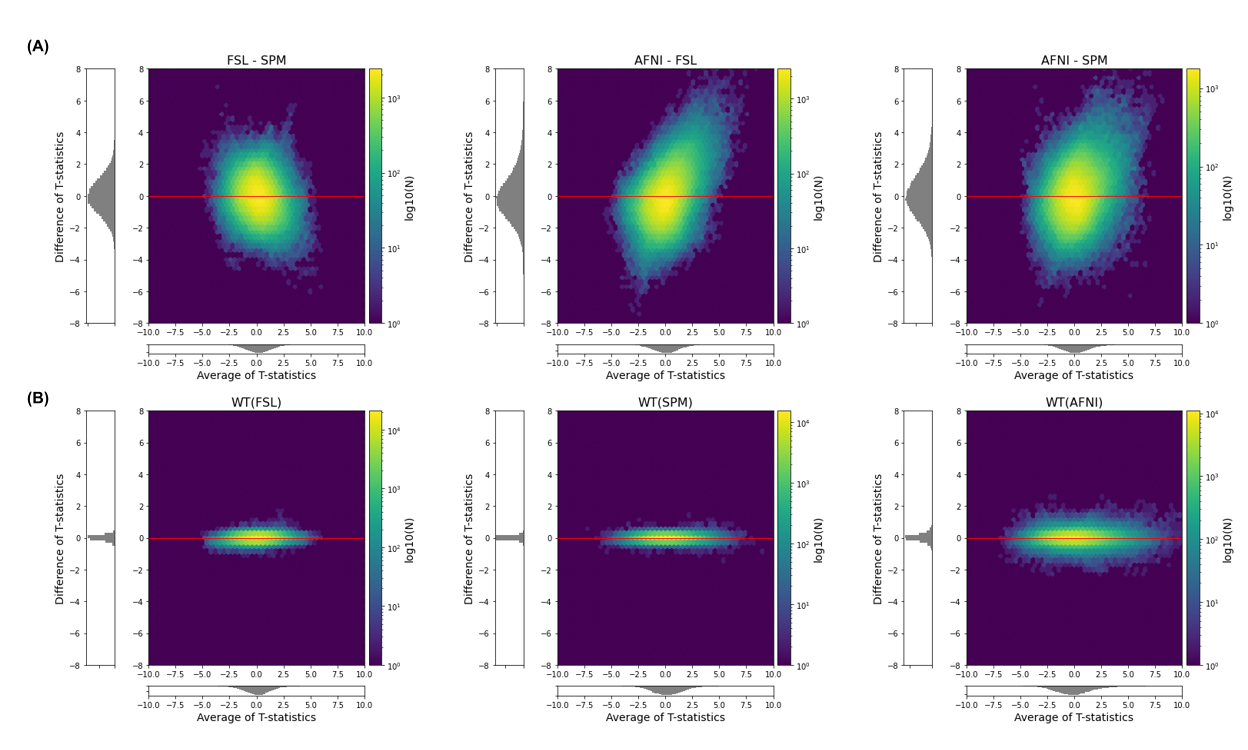
\includegraphics[width=.9\textwidth]{chapters/chapter3/figures/unthresh-gl-frame-fixedmask.png}
  \caption{\textbf{A} and \textbf{B}: Bland-Altman plots comparing group-level differences computed over the intersections 
  between tools (\textbf{A}) and within tools at machine error (\textbf{B}).}% \textbf{C}: voxel-wise comparison of absolute differences.}
  \label{fig:unthresh-maps-mask}
\end{figure*}

\section{Discussion}

In fMRI group analyses, within-tool software variability remains an order
of magnitude smaller than between-tool variability. This is likely
explained by the fact that group analyses benefit from regularization of
numerical noise, which is expected to increase with sample size. This finding is
consistent with observations made in~\cite{kiar2020numerical} from
diffusion MRI data where connectome graph statistics were found to be
substantially unstable at the subject level while group distributions
remained consistent. Therefore,
for fMRI studies with large sample sizes, within-tool software variability
may be neglected with respect to between-tool variability. In particular,
multiverse analyses aggregating the outcome of multiple analysis tools are
likely to successfully correct for machine error in such group studies.  Nevertheless, within-tool software variability remains
substantial in group analyses that are based on a single tool, as is
commonly the case in current fMRI studies. In particular, in our study, the
inherent instability of thresholding was triggered by within-tool software
variability in 20\% of 360 brain regions, which indicates that it might have
impacted neuroscientific conclusions related to these regions.

In subject-level analyses, within- and between-tool software variabilities can become
of comparable magnitude for some subjects in some regions. This observation
% can be used as a proxy for data quality, and
is particularly relevant to the development of fMRI-based biomarkers aiming
at individualized phenotype predictions. Machine error may play
a non-negligible role in such analyses, even when predictions combine
results produced by multiple tools.

For both group- and subject-level analyses, between- and within-tool
software variabilities similarly trigger the brain masking instability.
Even though both types of variability are different in nature, this result suggests
that in some cases they may have a common cause that might be related to
the conditioning of fMRI analysis in a specific dataset. 
% Along these lines,
% in some regions, instabilities of similar magnitude may be triggered by
% small numerical perturbations, model variations, or implementation
% differences. For instance, high-motion datasets may trigger between- and
% within-tool instabilities similarly. 

Therefore, numerical stability may be a suitable proxy to study
between-tool variability. This speculation might be of practical value to
address software variability at large given that within-tool variability
measurements can be automated while between-tool ones require substantial
human intervention. Indeed, within-tool variability can be simulated
irrespective of the particular analysis done, and with important sample
sizes, while between-tool variability requires re-implementing analysis in
different toolboxes and is limited to a few samples. Automated multi-verse
frameworks could be developed to assess and possibly reduce within-tool
variability as a pre-requisite for between-tool variability.

Our results are limited by the type of numerical noise introduced in the
analyses. Indeed, we only perturbed the outputs of elementary
mathematical functions while numerical noise could creep in any
floating-point operation. Therefore, our estimation of within-tool software variability should
be considered a lower bound. Likewise, our estimation of tool varability is
likely to be underestimated, having tested only 3 analytical pipelines
among the thousands available~\cite{carp2012plurality}.

In conclusion, our results motivate further numerical stability
investigations in fMRI analyses. Pipeline-level analyses could be conducted
to identify specific components that contribute to numerical variability,
and if possible correct them accordingly. Besides, in cases where
instability is inherent to the analysis, sampling results distributions
through numerical perturbations might improve stability, as explored
in~\cite{kiar2021data}. Finally, pipeline-specific statistical corrections
might be envisaged to account for within-tool software variability.

      
  \clearpage

\setcounter{equation}{0}
\setcounter{figure}{0}
\setcounter{table}{0}
\setcounter{section}{0}

\makeatletter
\renewcommand{\theequation}{S\arabic{equation}}
\renewcommand{\thefigure}{S\arabic{figure}}
\renewcommand{\thesection}{S\arabic{section}}

\textbf{\centering \Large Supplemental Materials}

\section{Reproduced results}
\label{sec:supp-repro}

Figure~\ref{fig:replication-diff} shows the difference in SPM and AFNI
group analyses maps between the results in~\cite{bowring2019exploring} and
our replication. Numerical perturbations of 1 ulp are likely to have been
introduced by our replication due to the use of GNU/Octave vs MATLAB for SPM
and multithreading for AFNI.
However, the group maps remained very similar
overall, which led us to conclude that our results correctly reproduced
the ones in~\cite{bowring2019exploring}.
\begin{figure*}[ht]
  % \fbox{\begin{minipage}{\dimexpr \textwidth-2\fboxsep-2\fboxrule}
  % \centering
  % \includegraphics[width=\textwidth]{figures/replication-diffs.png}
  \includegraphics[width=\textwidth]{chapters/chapter3/figures/replication-diffs.png}
  \caption{Differences between reproduced and original results obtained in~\cite{bowring2019exploring}
    of unthresholded group-level t-statistic for SPM (left) and AFNI
    (right). The highest areas of difference in AFNI seem to be due to
    differences in brain masks.}
  \label{fig:replication-diff}
  % \end{minipage}}
\end{figure*}


% \section{BT and WT correlations for all subjects}
% \label{sec:supp-subjects}

% Figure~\ref{fig:unthresh-correlation-allsbj} plots the relationship between
% WT and BT for each subject, showing a consistent moderate correlation between BT and
% WT.

% \begin{figure*}[ht]
%   \centering
%   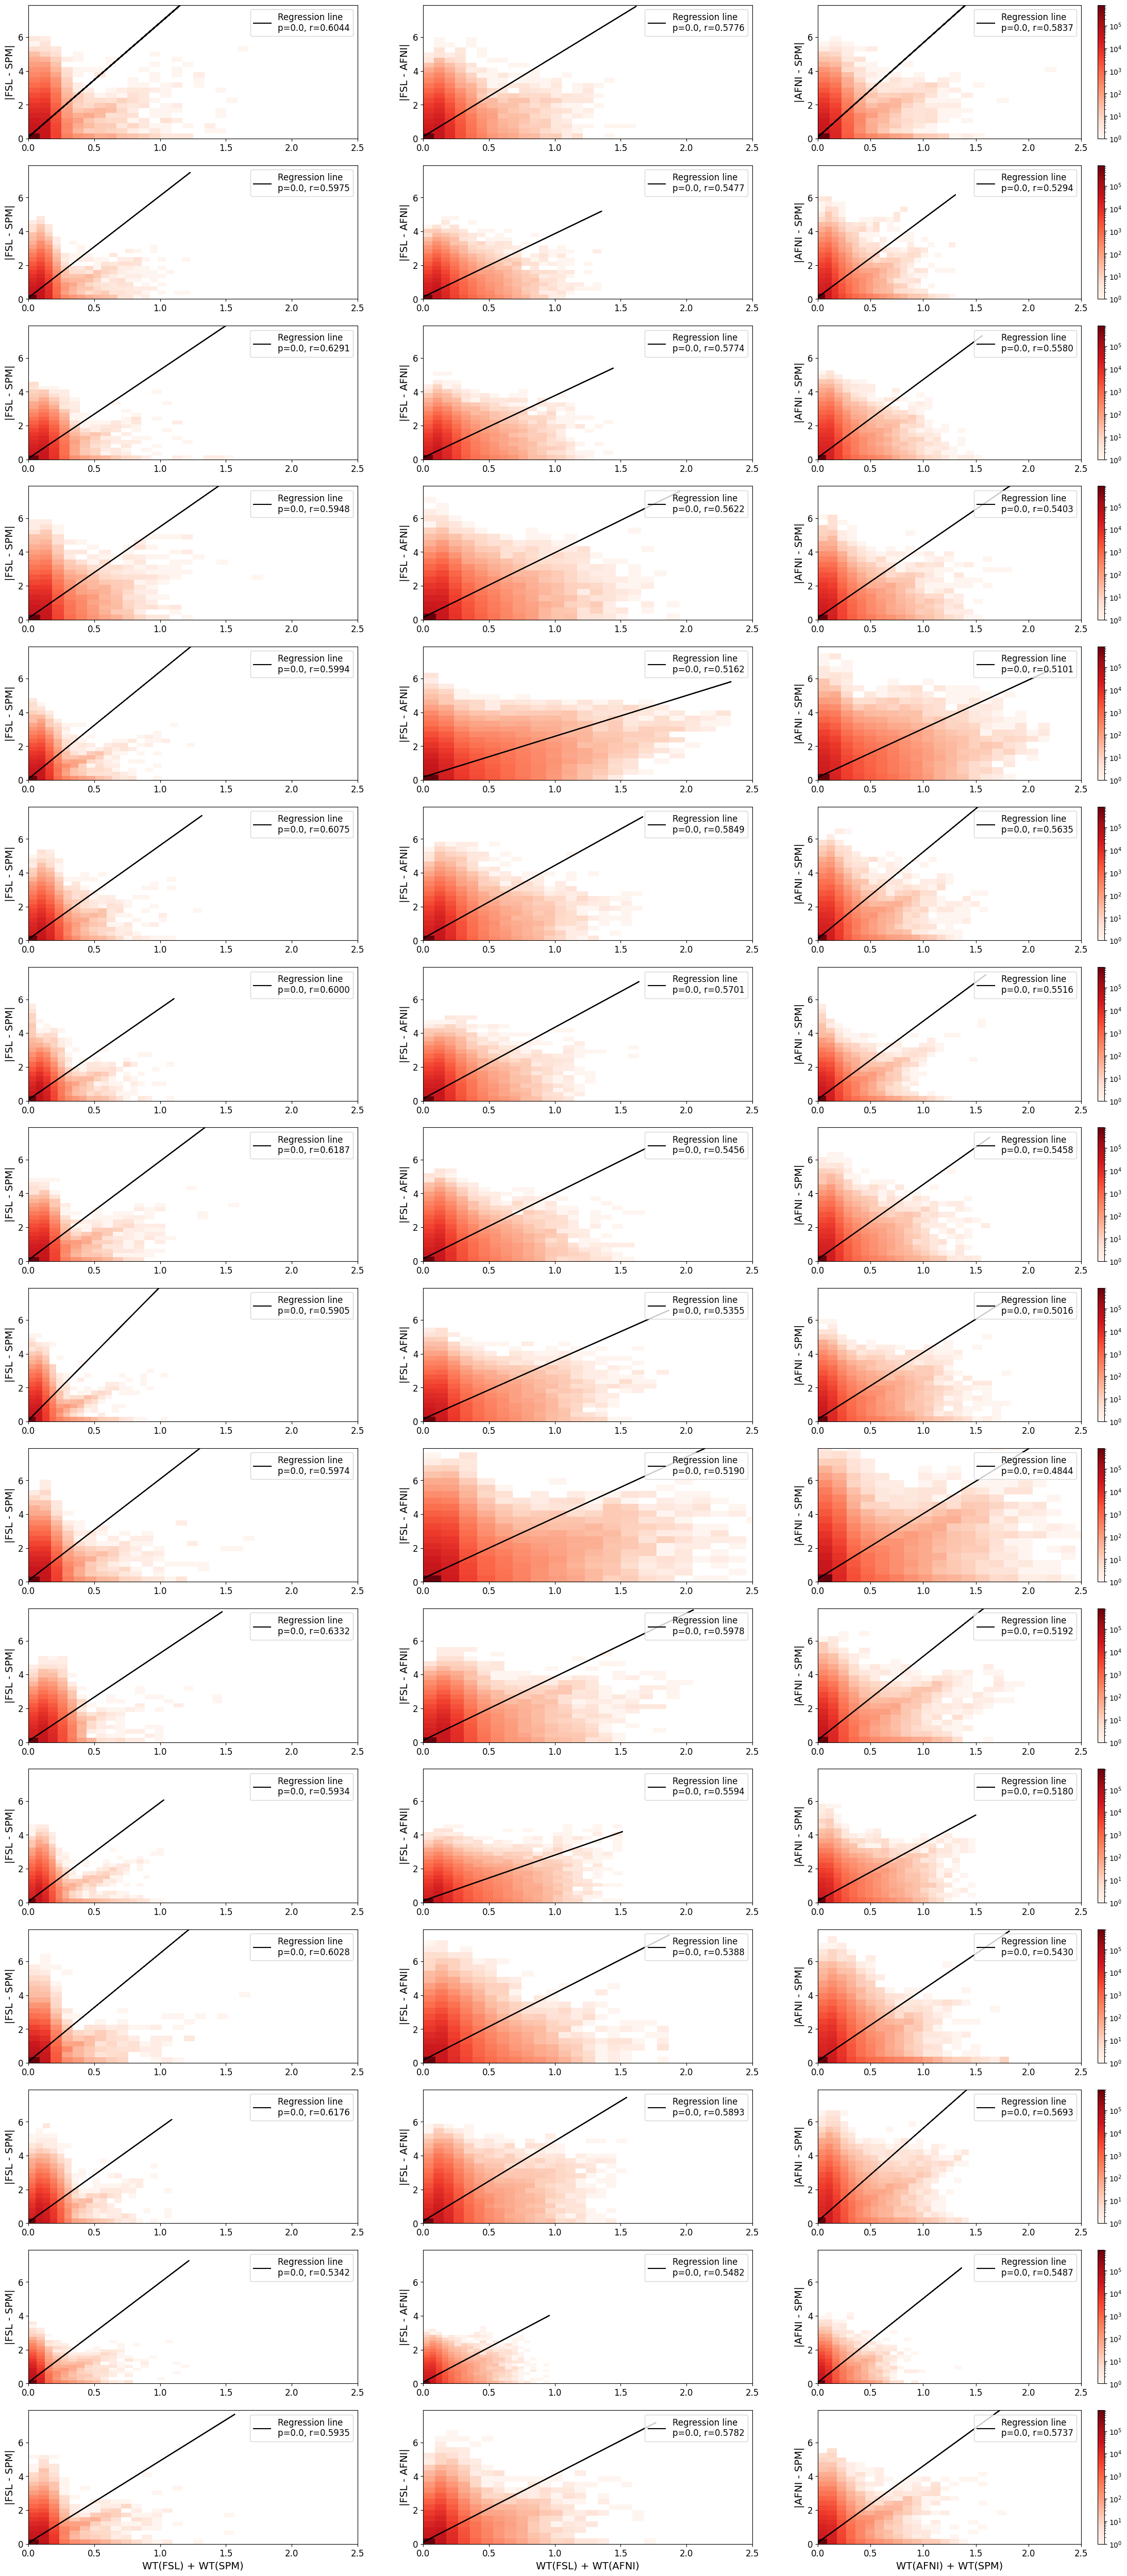
\includegraphics[width=.55\textwidth]{chapters/chapter3/figures/sbj-abs-corr-unthresh-plot.png}
%   \caption{Comparison between BT and WT variabilty for 16 subjects.}
%   \label{fig:unthresh-correlation-allsbj}
% \end{figure*}

\section{Maps of t-statistics for subject with highest WT variability}
\label{sec:supp-worst-subject}

Figure~\ref{fig:unthresh-worst-sbj} plots the maps of t-statistic
for each run of tools for the subject with highest WT variability.

\begin{figure*}[ht]
  \centering
  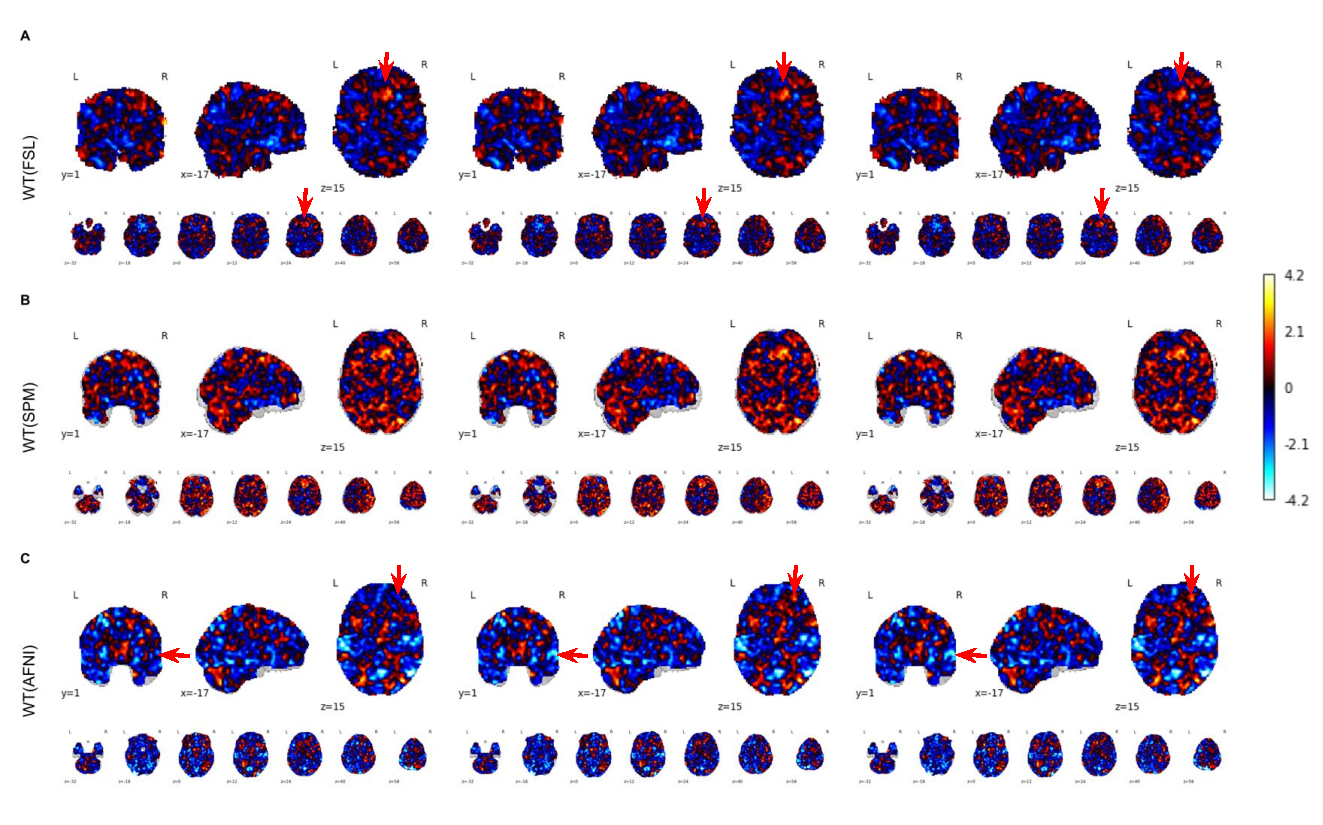
\includegraphics[width=\textwidth]{chapters/chapter3/figures/5-marked.pdf}
  \caption{For subject with highest WT variability, unthresholded subject-level t-statistic
  within tools at machine error for FSL (\textbf{A}),
  SPM (\textbf{B}), AFNI (\textbf{C}).}% \camille{If I understand correctly the point you are making here is that WT(AFNI) at some voxels is close to AFNI-SPM ? What is surprising here for me is that WT(AFNI) seems to be quite different from WT(SPM) and WT(FSL). Do we have a good idea why? Maybe looking at the maps would help?}
  %\ali{We are pointing regions with instability in both WT and BT, and yes indeed it shows a very different WT(AFNI) compare to WT(FSL) and WT(SPM), but we did not investigate the reason of variabilities for now.} }
  \label{fig:unthresh-worst-sbj}
\end{figure*}

